\documentclass[10pt]{article}

\usepackage[margin=1in]{geometry}
\setlength{\tabcolsep}{18pt}
\renewcommand{\arraystretch}{1.5}
\usepackage[table]{xcolor}
\usepackage{fontspec} 
\usepackage{graphicx}
\setmainfont{Arial}
\graphicspath{ {./Schemas/} }

\begin{document}
	
	\begin{titlepage} % Suppresses displaying the page number on the title page and the subsequent page counts as page 1
		\newcommand{\HRule}{\rule{\linewidth}{0.5mm}} % Defines a new command for horizontal lines, change thickness here
		
		\center % Centre everything on the page
		
		%------------------------------------------------
		%	Headings
		%------------------------------------------------
		
		\textsc{\LARGE Universita' degli studi di Padova}\\[1.5cm] % Main heading such as the name of your university/college
		
		\textsc{\Large D4C Cinemas}\\[0.5cm] % Major heading such as course name
		
		
		%------------------------------------------------
		%	Title
		%------------------------------------------------
		
		\HRule\\[0.4cm]
		
		{\huge\bfseries Progetto Basi di Dati}\\[0.2cm] % Title of your document
		
		\HRule\\[1.5cm]
		
		%------------------------------------------------
		%	Author(s)
		%------------------------------------------------
		
		\begin{minipage}{0.4\textwidth}
			\begin{flushleft}
				\large
				Damiano \textsc{Bertoldo} % Your name
			\end{flushleft}
		\end{minipage}
		~
		\begin{minipage}{0.4\textwidth}
			\begin{flushright}
				\large
				Alessandro \textsc{Canel} % Supervisor's name
			\end{flushright}
		\end{minipage}
		
		% If you don't want a supervisor, uncomment the two lines below and comment the code above
		{\large\textit{}}\\
		\textsc{2019/2020} % Your name
		
		%------------------------------------------------
		%	Date
		%------------------------------------------------
		
		\vfill\vfill\vfill % Position the date 3/4 down the remaining page
		
		
		%------------------------------------------------
		%	Logo
		%------------------------------------------------
		
		%\vfill\vfill
		%\includegraphics[width=0.2\textwidth]{placeholder.jpg}\\[1cm] % Include a department/university logo - this will require the graphicx package
		
		%----------------------------------------------------------------------------------------
		
		\vfill % Push the date up 1/4 of the remaining page		
		\tableofcontents
	\end{titlepage}
	\section{Abstract}	
	La societa' D4C Cinemas e' una catena di cinema, nata in regno unito nel 1988 da una partnership tra Universal Studios e Paramount Pictures che nel corso degli anni si e' estesa sia nel campo nazionale, che nel campo internazionale. Si vuole gestire la base di dati del cinema, comprendente la gestione di piu' cinema contemporaneamente. Ogni cinema e' un multisala contenente dalle 5 alle 10 sale ed ogni sala ha dai 150 ai 250 posti. D4C Cinemas rilascia giornalmente la programmazione degli spettacoli in modo tale da dare ai clienti varia scelta per l'orario. Una persona per acquistare un biglietto deve recarsi alla biglietteria e al momento dell'acquisto comunicare le credenziali, perche' il biglietto e' nominativo a differenza di altri cinema. Altra caratteristica di questa catena e' che al momento dell'uscita dalla sala lo spettatore puo' lasciare una recensione a caldo del film appena visto cosi' da lasciare ai futuri spettatori informazioni sul film. Altra cosa che viene effettuata in questa catena e' l'aggiunta e il tracciamento dei cast presenti, in modo tale da dare al clinte la possibilita' di avere la lista di film in cui recita il proprio attore/regista/sceneggiatore/produttore preferito.
	\section{Analisi dei requisiti}
	
	Il progetto vuole rappresentare una base di dati che permetta di gestire la programmazione dei film della catena UCI cinema.
			
	Essendo UCI cinemas una catena, e' necessario identificare la localita' di ciascun {\bf Cinema}:
	\begin{itemize}
		\item Nome cinema
		\item Quantita' sale
		\item Indirizzo, cosi' composto: via, citta', provincia, codice postale, regione, nazione
	\end{itemize}
	Per poter identificare una {\bf Sala} all'interno del cinema abbiamo bisogno delle sguenti informazioni:
	\begin{itemize}
		\item Numero sala (univoco all'interno del cinema)
		\item Cinema di appartenenza
		\item Numero posti
		\item Grandezza schermo (espresso in pollici)
	\end{itemize}
	All'interno di ogni sala viene proiettato un {\bf Film}:
	\begin{itemize}
		\item Titolo
		\item Durata
		\item Trama
		\item Genere
		\item Anno
	\end{itemize}
	Per conoscere il cast del film abbiamo bisogno di definire \textbf{Cast}:
	\begin{itemize}
		\item Film
		\item Lavoratore
	\end{itemize}
	Inoltre c'e' bisogno di conoscere il nome e il ruolo delle persone che ne hanno preso parte, e si possono suddividere in:
	\begin{itemize}
		\item {\bf Attore}: persona che ha recitato nel film 
		\item {\bf Sceneggiatore}: persona che ha strutturato la sceneggiatura del film 
		\item {\bf Produttore}: persona che ha finanziato il film 
		\item {\bf Regista}: persona che ha diretto il film
	\end{itemize}		 
	Di conseguenza abbiamo bisogno di definire {\bf Lavoratore}. Essendoci possibilita' di omonimia con stessa data di nascita, si preferisce utilizzare un identificativo:
	\begin{itemize}
		\item Id
		\item Nome
		\item Cognome
		\item Data di nascita
		\item Indirizzo, cosi' composto: via, citta', provincia, codice postale, regione, nazione
	\end{itemize}
	Il cinema per emettere i biglietti non ha bisogno delle credenziali del cliente, di conseguenza il bilgietto non e' nomintivo. Il {\bf Biglietto} ha le seguenti caratteristiche:
	\begin{itemize}	
		\item Film (film di interesse)
		\item Data e ora proiezione
		\item Cinema (dove viene proiettato il film)
		\item Sala
		\item Posto (scelto dall'utente al momento dell'acquisto)
	\end{itemize}
 	Per massimizzare l'utilizzo delle sale viene creata una \textbf{Programmazione} in cui vengono specificati gli orari di inizio dei vari film per i vari giorni, quindi sono necessarie le seguenti informazioni:
 	\begin{itemize}
 		\item Cinema
 		\item Sala
 		\item Film
 		\item Data e ora proiezione
 	\end{itemize} 
 	\subsection{Lista delle operazioni}		
	\textbf{Operazione 1}: Aggiuta di uno spettacolo per la proiezione di un film in una sala (40 volte al giorno) \\
	\textbf{Operazione 2}: Emissione biglietti (2500 volte al giorno)\\
	\textbf{Operazione 3}: Aggiunta nuovi film (5 volte al mese)\\
	\textbf{Operazione 4}: Rilascio di una recensione (2200 volte al giorno)\\
	\textbf{Operazione 5}: Aggiunta di un nuovo cast (4 volte al mese)\\
	\textbf{Operazione 6}: Conteggio totale posti venduti per ogni spettacolo (1 volta a settimana)
 	\subsection{Glossario dei termini}
 	\begin{tabular}{ |p{3cm}|p{4.5cm}|p{2.5cm}|p{3cm}|  }
 		%\hline
 		%\multicolumn{4}{|c|}{\textbf{Glossario dei termini}} \\
 		\hline
 		\rowcolor{lightgray}
 		\textbf{Termine} & \textbf{Descrizione} & \textbf{Sinonimi} & \textbf{Collegamenti} \\
 		\hline
 		Programmazione                         & Pianificazione orario inizio film all'interno del cinema                &                                                                                      & Film, Sala, biglietto                                                             \\ \hline
 		Sala                                   & Stanza dove viene proiettato il Film                                    &                                                                                      & Programmazione, Cinema \\ \hline
 		Biglietto                              & Acquisto del cliente, che attesta la vendita del posto per un dato film &                                                                                      & Programmazione \\ \hline
 		Lavoratore                                & Persona singola che ha preso parte alla realizzazione di almeno un Film                  & Attore, Sceneggiatore, Produttore, Regista & Cast                                                                        \\ \hline
 		Film                                   & Film presenti al cinema                                                 &                                                                                      & Programmazione, Biglietto, Cast        \\ \hline
 		Cinema                                   &    Impresa che offre il servizio cinematografico &                                                                                      & Sala        \\ \hline
 		Cast                                   &    Cast del film &                                                                                      & Film, Lavoratore        \\ \hline
 	\end{tabular}
 	\subsection{Strutturazione dei requisiti}
	\begin{tabular} { |p{16.8cm}| }
 		\hline
 		\rowcolor{lightgray}
 		\textbf{Frasi relative a "Cinema"} \\
 		\hline
 		I Cinema vengono identificati tramite: Nome cinema, Quantita' sale, Indirizzo (composto da via, citta', provincia, codice postale, regione, nazione) \\
 		\hline 		
 	\end{tabular}
 	\\\\\\
	\begin{tabular} { |p{16.8cm}| }
	 	\hline
	 	\rowcolor{lightgray}
	 	\textbf{Frasi relative a "Sala"} \\
	 	\hline
	 	Le Sale vengono identificate tramite: Numero sale (univoco all'interno del cinema), Numero posti, Cinema di appartenenza, Grandezza schermo (espresso in pollici) \\
	 	\hline 		
	\end{tabular} 
	\\\\\\
	\begin{tabular} { |p{16.8cm}| }
		\hline
		\rowcolor{lightgray}
		\textbf{Frasi relative a "Film"} \\
		\hline
		I Film vengono identificati tramite: Titolo, Durata, Trama, Genere, Anno \\
		\hline 		
	\end{tabular} 
 	\\\\\\
 	\begin{tabular} { |p{16.8cm}| }
 		\hline
 		\rowcolor{lightgray}
 		\textbf{Frasi relative a "Cast"} \\
 		\hline
 		Il Cast viene identificato tramite: Film, Lavoratore \\
 		\hline 		
 	\end{tabular} 
 	\\\\\\
 	\begin{tabular} { |p{16.8cm}| }
 		\hline
 		\rowcolor{lightgray}
 		\textbf{Frasi relative a "Lavoratore"} \\
 		\hline
 		I Lavoratori vengono identificati tramite: Id, Nome, Cognome, Data di nascita, indirizzo (composto da via, citta', provincia, codice postale, regione, nazione) \\
 		\hline 		
 	\end{tabular} 
 	\\\\\\
 	\begin{tabular} { |p{16.8cm}| }
 		\hline
 		\rowcolor{lightgray}
 		\textbf{Frasi relative a "Attore"} \\
 		\hline
 		Persona che ha lavorato come attore nel film \\
 		\hline 		
 	\end{tabular} 
	\\\\\\
	\begin{tabular} { |p{16.8cm}| }
		\hline
		\rowcolor{lightgray}
		\textbf{Frasi relative a "Sceneggiatore"} \\
		\hline
		Persona che ha lavorato come sceneggiatore nel film \\
		\hline 		
	\end{tabular} 
	\\\\\\
	\begin{tabular} { |p{16.8cm}| }
		\hline
		\rowcolor{lightgray}
		\textbf{Frasi relative a "Produttore"} \\
		\hline
		Persona che ha lavorato come produttore nel film \\
		\hline 		
	\end{tabular} 
	\\\\\\
	\begin{tabular} { |p{16.8cm}| }
		\hline
		\rowcolor{lightgray}
		\textbf{Frasi relative a "Regista"} \\
		\hline
		Persona che ha lavorato come regista nel film \\
		\hline 		
	\end{tabular} 
	\\\\\\
	\begin{tabular} { |p{16.8cm}| }
		\hline
		\rowcolor{lightgray}
		\textbf{Frasi relative a "Biglietto"} \\
		\hline
		I Biglietti vengono idetificati tramite: Film, Data e ora proiezione, Cinema, Sala, Posto \\
		\hline 		
	\end{tabular} 
	\\\\\\
	\begin{tabular} { |p{16.8cm}| }
		\hline
		\rowcolor{lightgray}
		\textbf{Frasi relative a "Programmazione"} \\
		\hline
		La Programmazione viene idetificata tramite: Cinema, Sala, Film, Data e ora proiezione \\
		\hline 		
	\end{tabular} 
	
	\section{Progettazione Concettuale}	
	\subsection{Lista delle entita'}
	Di seguito veranno riportate le classi che verranno contenute nel database, tutti i campi sono \textbf{not null} tranne quelli specificati.\\
	\underline{Gli identificatori delle entita' sono sottolineati.}
	\begin{itemize}
		\item \textbf{Cinema}: Rappresenta un cinema.
		\begin{itemize}
			\item \underline{Nome: \textit{string} univoco}
			\item Numero sale: \textit{int}
			\item Indirizzo: attributo composto
				\subitem Via: \textit{string}
				\subitem Citta': \textit{string}
				\subitem Provincia: \textit{string}
				\subitem CAP: \textit{int}
				\subitem Regione: \textit{string}
				\subitem Nazione: \textit{string}			
		\end{itemize}
		\item \textbf{Sala}: Rappresenta una sala di un cinema.
		\begin{itemize}
			\item \underline{Sala: \textit{int}}
			\item \underline{Cinema: \textit{string}}
			\item Numero\_posti: \textit{int}
			\item Grandezza\_schermo: \textit{int}
		\end{itemize}
		\item \textbf{Film}: Rappresenta un film.
		\begin{itemize}
			\item \underline{Titolo: \textit{string}}
			\item \underline{Anno: \textit{int}}
			\item Durata: \textit{timestamp}
			\item Genere: \textit{string}
			\item Trama: \textit{string}
		\end{itemize}
		\item \textbf{Lavoratore}: Rappresenta una persona che ha preso parte alla realizzazione di almeno un film.
		\begin{itemize}
			\item \underline{Id: \textit{int} univoco}
			\item Nome: \textit{string}
			\item Cognome: \textit{string}
			\item Data\_di\_nascita: \textit{datetime}			
			\item Indirizzo: attributo composto, possibile \textit{null}
				\subitem Via: \textit{string}
				\subitem Citta': \textit{string}
				\subitem Provincia: \textit{string}
				\subitem CAP: \textit{int}
				\subitem Regione: \textit{string}
				\subitem Nazione: \textit{string}
		\end{itemize}
	\end{itemize}
	\section{Progettazione logica}
	\subsection{Analisi ridondanza}	
	Una ridondanza si trova nell'entita' \textbf{Spettacolo}, nella quale l'attributo \textbf{posti\_venduti} si puo' calcolare visitando la relazione \textbf{Spettacolo-Biglietto} (chiamata "fa riferimento") e contando le occorrenze di tale relazione.
	\begin{table}[!h]
		\centering
		\begin{tabular}{|c|c|c|}
			\hline
			\textbf{Concetto} & \textbf{Tipo} & \textbf{Volume} \\
			\hline
			Spettacolo & E & 200 \\
			\hline
			Biglietto & E & 28000 \\
			\hline
			Fa' Riferimento & R & 28000 \\
			\hline
		\end{tabular}
	\end{table}
	\begin{itemize}
		\item \textbf{Operazione 2}: Emissione biglietti (2500 volte al giorno)
		\item \textbf{Operazione 6}: Conteggio totale posti venduti per ogni spettacolo (1 volta a settimana)		
	\end{itemize}
	L'operazione 6 ha come scopo contare l'affluenza settimanale dei clienti.\\
	Di seguito le operazioni di conteggio in scrittura verranno considerate doppie perche' operazioni piu onerose rispetto alle operazioni di lettura.
	\subsubsection{Presenza di ridondanza}
	L'attributo \textbf{posti\_venduti}, cosi' come indicato nello schema ER, indica il numero totale di posti venduti per uno spettacolo.
	\begin{table}[h!]
		\centering
		\caption{\textbf{Operazione 2}} \label{tab:sometab}
		\begin{tabular}{|c|c|c|c|}
			\hline
			\textbf{Concetto} & \textbf{Costrutto} & \textbf{Accessi} & \textbf{Tipo} \\
			\hline
			Biglietto & E & 1 & S \\
			\hline
			Fa' riferimento & R & 1 & S \\
			\hline
			Spettacolo & E & 1 & L \\
			\hline
			Spettacolo & E & 1 & S \\
			\hline
		\end{tabular}
		\begin{itemize}
			\item Costi 3*2500 + 1*2500 = 17500 accessi 
		\end{itemize}
		\caption{\textbf{Operazione 6}} \label{tab:sometab}
		\begin{tabular}{|c|c|c|c|}
			\hline
			\textbf{Concetto} & \textbf{Costrutto} & \textbf{Accessi} & \textbf{Tipo} \\
			\hline
			Spettacolo & E & 1 & L \\
			\hline
		\end{tabular}
		\begin{itemize}
		\item Costi 1*200 = 200 accessi 
		\end{itemize}
	\end{table}
	Il totale degli accessi, essendo l'operazione 2 giornaliera e l'operazione 6 settimanale, si calcola in questo modo: 17500*7 + 200 = 122700 accessi.
	\subsubsection{Assenza di ridondanza}
	In questo caso per calcolare i posti venduti senza l'attributo posti\_venduti, bisogna fare riferimento alla relazione \textbf{Spettacolo-Biglietto} (relazione di nome "Fa' riferimento") e contarne le rispettive occorrenze.	
	\begin{table}[h!]
		\centering
		\caption{\textbf{Operazione 2}} \label{tab:sometab}
		\begin{tabular}{|c|c|c|c|}
			\hline
			\textbf{Concetto} & \textbf{Costrutto} & \textbf{Accessi} & \textbf{Tipo} \\
			\hline
			Biglietto & E & 1 & S \\
			\hline
			Fa' riferimento & R & 1 & S \\
			\hline
		\end{tabular}
		\begin{itemize}
			\item Costi 2*2500 = 10000 accessi 
		\end{itemize}
		\caption{\textbf{Operazione 6}} \label{tab:sometab}
		\begin{tabular}{|c|c|c|c|}
			\hline
			\textbf{Concetto} & \textbf{Costrutto} & \textbf{Accessi} & \textbf{Tipo} \\
			\hline
			Spettacolo & E & 1 & L \\
			\hline
			Fa' riferimento & R &140&L\\
			\hline
		\end{tabular}
		\begin{itemize}
			\item Costi 1*200 + 140*200 = 28200 accessi
		\end{itemize}
	\end{table}
	Il totale degli accessi, essendo l'operazione 2 giornaliera e l'operazione 6 settimanale, si calcola in questo modo: 10000*7 + 28200 = 108200 accessi.\\\\
	In coclusione la ridondanza del dato non porta vantaggi, di conseguenza si e' deciso di eliminarla.
	\subsection{Ristrutturazione schema ER}
	\subsubsection{Eliminazione generalizzioni}
	\paragraph{Persona}
	La generalizzaione \textit{Persona}, rappresenta una persona che e' un cliente del cinema, ha come figlia l'entita' \textit{Lavoratore}, che in questo caso viene considerato come il lavoratore che prende parte alla realizzazione di un film.\\
	Essendo una generalizzazione parziale, si e' deciso di dividere le due entita' e creare una associazione uno a uno tra le due. Questo perche' ci sono occorrenze che riferiscono singolarmente con l'entita' figlia Lavoratore.\\
	\paragraph{Lavoratore}
	A sua volta la generalizzazione di \textit{Lavoratore} ha quattro entita' figlie: \textit{Attore}, \textit{Sceneggiatore}, \textit{Produttore} e \textit{Regista}.\\
	Essendo in questo caso una generalizzazione completa, e non essendoci associazioni dirette con le entita' figlie, si e' deciso di accorpare le entita' figlie all'interno dell'entita' \textit{Lavoratore}, aggiungendone un nuovo attributo \textit{Ruolo}, il quale ha lo scopo di identificare i vari ruoli svolti dal lavoratore.
	\subsubsection{Introduzione entita' indirizzo}
	Per rappresentare le informazioni sull’indirizzo riguardanti la posizione di un \textit{Cinema}, è stata introdotta l’entità \textit{Indirizzo}. Questa entità contiene i seguenti attributi: cap, via, numero civico, nazione e città. \textit{Cinema} sara' l'unica entita' collegata ad \textit{Indirizzo}.
	\subsubsection{Scelta degli identificatori primari}
	\paragraph{Cinema}
	Come scelta dell'identificatore primario nell'entita', viene scelto l'attributo \textit{Nome}, perche' il nome identifica un singolo cinema.
	\paragraph{Sala}
	Per identificare una sala, viene scelto come identificatore il numero della sala, \textit{numero}, e il cinema di appartenenza, \textit{Cinema}. Questo perche' all'interno del cinema il numero della sala e' univoco.
	\paragraph{Spettacolo}
	Per identificare uno spettacolo bisognerebbe fare riferimento all'attributo \textit{dataora\_inizio} insieme alla \textit{sala} e al \textit{film}. Quindi per semplicita' viene aggiunto un nuovo attributo identificatore \textit{Id}, cio' semplifica e rende meno ambigua l'identificazione di una tupla all'interno di spettacolo.
	\paragraph{Biglietto}
	Per identificare il singolo biglietto si ricorre all'utilizzo di un identificatore \textit{Id}, questo per la stessa motivazione presente in \textit{Spettacolo}.
	\paragraph{Film}
	Per identificare un singolo film, bisognerebbe comprendere \textit{Titolo, Anno, Genere e Durata}, dato che potrebbe verificarsi l'uscita di un film omonimo nello stesso anno con lo stesso genere. Quindi per semplificare e rendere ancora piu' forte l'identificazione, viene introdotto l'attributo identificatore \textit{Id}.
	\paragraph{Recensione}
	Per identificare la singola recensione si utilizza \textit{Persona e Film}, dato che la coppia ne identifica una tupla.
	\paragraph{Persona}
	Per identificare una persona, \textit{Nome, Cognome e Data\_nascita} possono risultare inadeguati, quindi viene introdotto l'attributo identificatore \textit{Id}.
	\paragraph{Lavoratore}
	Per identificare un lavoratore, viene utilizzato il suo \textit{Ruolo}, il riferimento a persona \textit{Persona} e la sua presenza ad un \textit{Cast}, questo perche' un lavoratore puo' assumere piu' ruoli all'interno di un cast.
	\paragraph{Cast}
	Per identificare un cast si ricorre all'utilizzo di un identificatore \textit{Id}, questo perche' potrebbero esserci cast omonimi.
	\paragraph{Indirizzo}
	Per identificare un indirizzo si ricorre all'utilizzo di un identificatore \textit{Id}, questo per minimizzare l'utilizzo di attributi per il riconoscimento della singola tupla.
	\subsubsection{Schema ER ristrutturato}	
	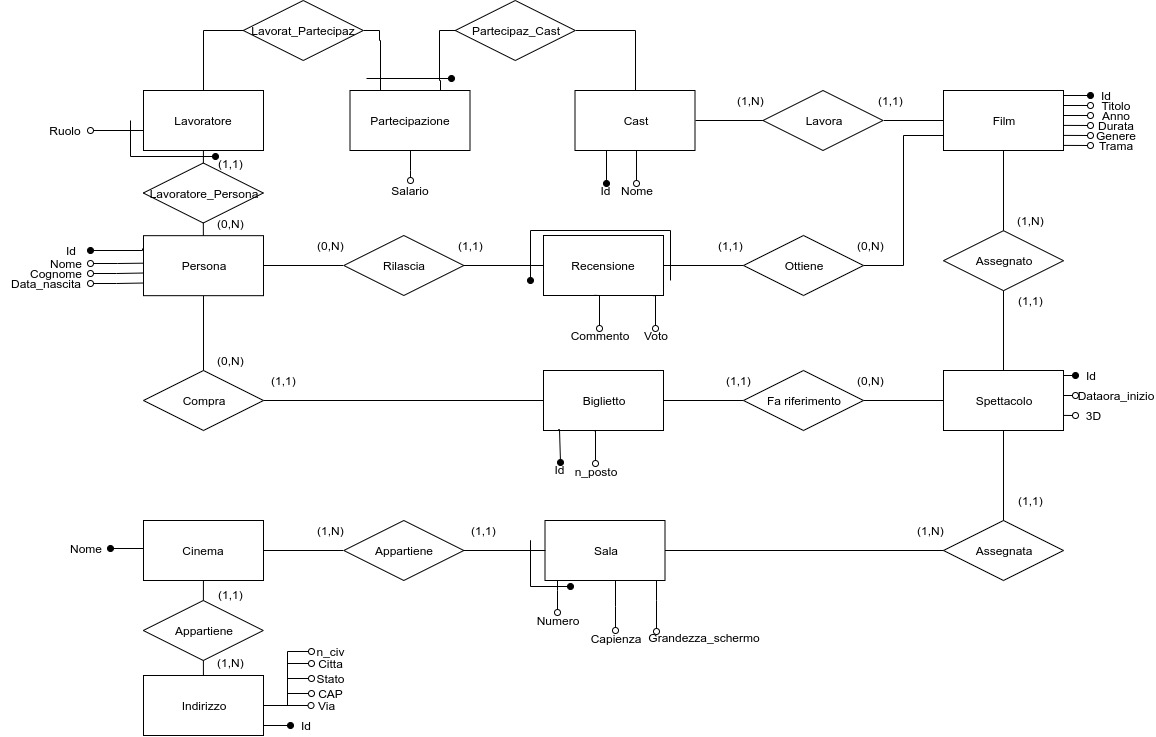
\includegraphics[height=\textwidth, width=23cm, angle=90]{SchemaER_Rev}
	\subsection{Traduzione nel modello relazionale}
	\textbf{Cinema}(\underline{Nome}, Indirizzo)\\
	\textit{vincolo di integrita' referenziale tra "Indirizzo" ed "Id" in Indirizzo.}\\\\
	\textbf{Sala}(\underline{Numero}, \underline{Cinema}, Capienza, Grandezza\_schermo)\\
	\textit{Vincolo di integrita' referenziale tra "Cinema" e "Nome" in Cinema.}\\\\
	\textbf{Spettacolo}(\underline{Id}, Dataora\_inizio, 3D, Film, Sala, Cinema)\\
	\textit{Vincolo di integrita' referenziale tra "Film" ed "Id" in Film, "Sala" e "Id" in Sala e tra "Cinema" e "Cinema" in Sala.}\\\\
	\textbf{Biglietto}(\underline{Id}, n\_posto, Spettacolo, Persona)\\
	\textit{Vincolo di integrita' referenziale tra "Spettacolo" ed "Id" in Spettacolo e tra "Persona" e "Id" in Persona.}\\\\
	\textbf{Film}(\underline{Id}, Titolo, Anno, Durata, Genere, Trama, Cast)\\
	\textit{Vincolo di integrita' referenziale tra "Cast" e "Id" in Cast}.\\\\
	\textbf{Recensione}(\underline{Film}, \underline{Persona}, Commento, Voto)\\
	\textit{Vincolo di integrita' referenziale tra "Film" e "Id" in Film e tra "Persona" e "Id" in Persona.}\\\\
	\textbf{Persona}(\underline{Id}, Nome, Cognome, Data\_nascita)\\\\
	\textbf{Lavoratore}(\underline{Persona}, \underline{Cast}, \underline{Ruolo}, Salario)\\	
	\textit{Vincolo di integrita' referenziale tra "Persona" e "Id" in Persona e tra "Cast" e "Id" in Cast}.\\\\
	\textbf{Cast}(\underline{Id}, Nome).\\\\
	\textbf{Indirizzo}(\underline{Id}, Via, Citta, n\_civ, Stato, Cap)\\\\
\end{document} 
